\documentclass{article} 
\UseRawInputEncoding
\usepackage[utf8]{inputenc}
\usepackage[T1]{fontenc}
\usepackage{selinput}
\usepackage[spanish]{babel}
\usepackage{hyphenat}
\usepackage{graphicx} 
\usepackage{subcaption}
\usepackage{hyperref}
\usepackage{listings}
\usepackage{xcolor}
\usepackage{float}
\begin{document}
\date{} 

\begin{center}
    
\includegraphics[width=1\textwidth]{Imagenes/Logo/LogoBIASbn.png}\\ 
\end{center}

\title{}

\vspace{1cm} 

\textbf{Integrantes del Proyecto:} 

\begin{itemize}
    \item Adell, Nicolas Fabian
    \item De Blasi, Luca
    \item Diaz Melion, Danilo Sebastian
    \item Gil Soria, Ian Lucas
    \item Montenegro, Luciano Nahuel
    \item Sojka, Santiago Alejandro
\end{itemize}

\tableofcontents 

\newpage 

\section{Introducción}
El proyecto BIAS es un módulo diseñado para su aplicación en sillas de ruedas, permitiendo al usuario dirigirla mediante el control mental, es decir, a través de sus pensamientos. Con este enfoque, se elimina la necesidad de utilizar un control físico, como el joystick empleado en las sillas eléctricas convencionales. De esta manera, se ofrece mayor independencia y una mejor calidad de vida a personas con movilidad reducida, como aquellos que padecen esclerosis lateral amiotrófica (ELA).


Para su funcionamiento, BIAS emplea una Inteligencia Artificial desarrollada por nuestro equipo, capaz de reconocer los patrones de las señales cerebrales asociadas al movimiento. Estos patrones se traducen en acciones que permiten dirigir la silla en distintas direcciones o, si el usuario así lo desea, mantenerla en su posición actual.

\section{¿Quiénes somos?}
El equipo BIAS (Brain Intelligence Artificial System) está conformado por seis integrantes, todos estudiantes de la Escuela Técnica N° 7 "IMPA" de Quilmes. Actualmente, nos encontramos cursando el séptimo y último año de la educación secundaria, en la especialidad de Aviónica, más específicamente a la segunda división, comisión "C".


Dedicamos aproximadamente 30 horas semanales al desarrollo del proyecto, en el marco de la asignatura denominada "Profesionalizantes", donde destinamos todo el tiempo a esta actividad. En dicha materia, tenemos a cargo a tres profesores, quienes son:

\begin{itemize}
    \item Fabrizio Carlassara
    \item Sergio Medina
    \item Carlos Bianco
\end{itemize}

\subsection{Metodología de Trabajo}

La metodología aplicada en este proyecto se basa en la organización del equipo en dos grupos especializados. El primer grupo se encarga del desarrollo de los programas, siendo ejemplos de esto los filtros virtuales, programas de recepción y procesado, mientras que el segundo se dedica a la implementación de los motores, sistemas de emergencia y filtros. Esta división del trabajo permite una utilización más eficiente del tiempo, al abordar simultáneamente diversas áreas del proyecto, lo que resulta en un avance más significativo en periodos de tiempo más reducidos.

\section{¿Por qué hacemos este proyecto?}

Como estudiantes de séptimo año, nuestro objetivo es desarrollar un proyecto que cumpla con los requisitos de las prácticas profesionalizantes. Desde un principio, nos propusimos encontrar una iniciativa que generara un impacto social significativo, centrada en mejorar la calidad de vida de personas con discapacidades. En este contexto, y luego de investigar, pensamos en la idea de crear un módulo para sillas de ruedas controlado por la actividad cerebral del usuario, utilizando tecnología de interfaz cerebro-computadora (BCI).

\section{¿A quiénes está dirigido este proyecto?}
Este proyecto está dirigido a personas con movilidad reducida, especialmente aquellos pacientes que presentan una parálisis completa desde el cuello hacia abajo. Entre los principales beneficiarios se encuentran personas que padecen esclerosis lateral amiotrófica (ELA), cuadriplejia, esclerosis múltiple, o aquellos que han sufrido la amputación de extremidades. Dado que el control de la silla de ruedas se realiza a través de señales cerebrales, el alcance del proyecto puede extenderse a una amplia variedad de pacientes con limitaciones motrices de este tipo.


Estamos convencidos de que este proyecto tiene el potencial de transformar la vida de personas con movilidad reducida, permitiéndoles gestionar su propio movimiento y mejorando sustancialmente su calidad de vida.

\section{¿Por qué es innovador este proyecto?}

Consideramos que este proyecto es innovador debido a la escasez de opciones similares en el mercado, sumado a nuestro enfoque en hacerlo accesible para el mayor número posible de personas, facilitando su adquisición por aquellos que lo necesiten. Un aspecto clave de este proyecto es la integración de inteligencia artificial en su funcionamiento, lo que lo diferencia de las soluciones convencionales. Mientras que la mayoría de las sillas de ruedas disponibles se controlan mediante un joystick, esta sería una de las primeras en emplear señales cerebrales para su operación.

La inversión en tiempo y recursos adicionales permitirá perfeccionar sus características técnicas, optimizar su funcionalidad, y adaptar el producto a las necesidades de un mercado que se expande. Una vez finalizado y refinado, el proyecto podrá captar la atención de un público más amplio, lo que incrementará su viabilidad comercial y su posicionamiento en el mercado.

En caso de que el desarrollo del proyecto no se complete en su totalidad, este podrá ser aprovechado por la institución educativa, permitiendo que otros grupos de estudiantes continúen su avance. De esta manera, el proyecto no solo servirá como un recurso valioso para futuras generaciones, sino que también fomentará la colaboración y el aprendizaje continuo dentro de la comunidad académica, garantizando su evolución y finalización.

\section{Descripción del funcionamiento}
El usuario se sienta en la silla de ruedas y se coloca el dispositivo EEG. El EEG capta las señales cerebrales y las somete a un proceso de filtrado por hardware de varias etapas. Luego, las envía a un circuito de compensación de Offset, para que la RP2040 Zero pueda leerlas. Estos datos, se los envía a la Raspberry Pi 4, en donde está el programa principal de la silla de ruedas.

En esta placa se encuentran los filtros digitales, el programa para el control de los motores, el procesamiento de señales y la inteligencia artificial. Una vez que las señales llegan a la Raspberry Pi 4, se las filtra digitalmente para eliminar el ruido de las señales. Luego de ser filtradas, se las envía a la IA, que reconoce los patrones cerebrales, y dependiendo de a dónde se quiera mover el usuario, enviará una señal a los motores en la dirección deseada, ya sea hacia adelante, detrás, izquierda, derecha o mantenerse en el lugar.


\subsection {Informacion Adicional}
La silla desarrollada en este proyecto es un prototipo, es decir, puede contener fallas de todo tipo, y es sujeto a modificaciones a futuro. Se recomienda su uso siempre acompañado, en zonas amplias libres de obstáculos. No se debe usar en lugares húmedos o si el equipo está mojado, y la inteligencia artificial está adaptada a las muestras de una persona del equipo del proyecto, por lo que para ser usada por alguien mas se deberán muestrear los patrones de movimiento de esta misma.

En caso de que haya un error en la lectura de señales o haya un obstáculo en la trayectoria de la silla, se activará un sistema de emergencia. Su objetivo es prevenir accidentes y brindarle mayor seguridad al usuario. El sistema frena los motores y enciende un LED en la dirección del obstáculo, y enciende un buzzer, que enciende una señal sonora.

\subsubsection{¿Que es un EEG?}

Un electroencefalógrafo es un dispositivo médico que se utiliza para registrar y medir la actividad eléctrica del cerebro. Su función principal es captar las señales eléctricas generadas por las neuronas cerebrales y transformarlas en gráficos de ondas cerebrales, que se pueden analizar para evaluar la función cerebral.

\subsubsection{Componentes que tiene un EEG}
\begin{itemize}
    \item \textbf{Electrodos:} Pequeños sensores que se colocan en el cuero cabelludo para captar los cambios de voltaje producidos por la actividad cerebral.
    \item \textbf{Amplificador:} Como las señales eléctricas del cerebro son muy débiles, el electroencefalógrafo incluye amplificadores que aumentan la señal para que sea lo suficientemente fuerte como para ser registrada.
    \item \textbf{Conversor analógico-digital:} Convierte las señales eléctricas captadas en un formato digital para su procesamiento por computadora.
    \item \textbf{Software de procesamiento:} El dispositivo utiliza un software que transforma las señales en gráficos de ondas cerebrales que se presentan en tiempo real en una pantalla o se registran para análisis posterior.
    \item \textbf{Pantalla/Gráficos:} El electroencefalógrafo muestra las señales eléctricas en forma de ondas, conocidas como ondas cerebrales (Delta, Theta, Alpha, Beta, Gamma), lo que permite a los médicos interpretar la actividad cerebral.
\end{itemize}

\subsubsection{¿Cómo se aplican los electrodos?}

El sistema 10-20 es un método internacionalmente estandarizado para la colocación de electrodos en el cuero cabelludo durante un electroencefalograma (EEG). Este sistema asegura que los electrodos se coloquen de manera uniforme y precisa en relación con los puntos anatómicos del cráneo, permitiendo una medición consistente y reproducible de la actividad eléctrica cerebral.

El sistema 10-20 se utiliza para garantizar una colocación precisa y consistente de los electrodos en los estudios de EEG. Algunos de sus beneficios incluyen:

\begin{itemize}
    \item \textbf{Estandarización global:} Permite que los estudios de EEG sean comparables en diferentes laboratorios y entre diferentes pacientes.
    \item \textbf{Cobertura completa del cerebro:} El sistema asegura que se cubran adecuadamente diferentes áreas del cerebro (frontal, parietal, occipital, temporal).
    \item \textbf{Detección de anomalías:} Facilita la identificación de regiones del cerebro donde pueden estar ocurriendo fenómenos anormales, como descargas epilépticas, actividad lenta anormal o asimetrías en las ondas cerebrales.
\end{itemize}

El nombre "10-20" proviene de las distancias porcentuales entre los electrodos: Los electrodos se colocan en posiciones que están al 10\% o al 20\% de la distancia total entre puntos anatómicos clave del cráneo.
Puntos anatómicos clave de referencia:

\begin{itemize}

    \item \textbf{Nasion:} El punto entre la frente y la nariz.
    
    \item \textbf{Inion:} El punto más prominente en la parte posterior de la cabeza.
    
    \item \textbf{Puntos preauriculares:} Justo por encima de los oídos, a cada lado de la cabeza.
    
\end{itemize}

Las posiciones de los electrodos se distribuyen sobre la cabeza tomando como referencia estos puntos para cubrir todo el cuero cabelludo de forma equidistante.

\newpage

En la siguiente imágen se puede visualizar de mejor manera la posición de los electrodos:

\begin{figure}[H]

    \centering
    
    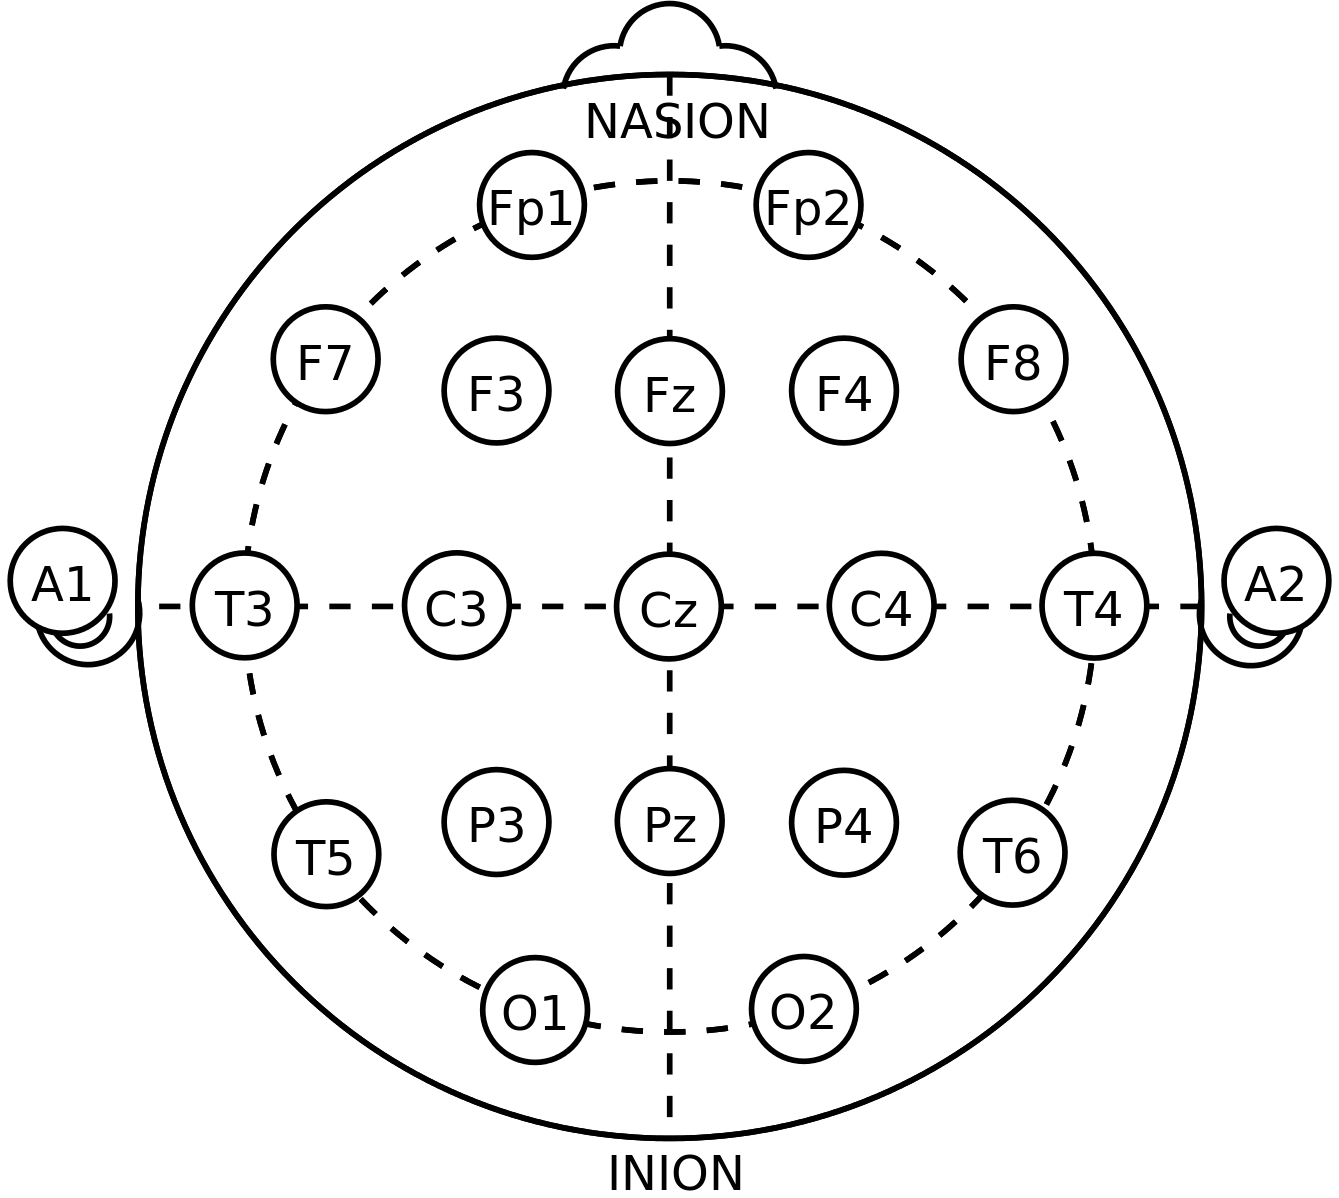
\includegraphics[width=0.7\linewidth]{Imagenes//Sistema10-20/localizacionelectrodoseeg.png}
    \caption{Sistema 10-20}
    
\end{figure}

\subsubsection{Pasos para aplicar el sistema 10-20}

\begin{enumerate}

    \item \textbf{Medición del cráneo:} Se mide la distancia desde el nasion al inion y desde un punto preauricular al otro. Luego, se calculan los puntos intermedios en un 10 o 20 de esas distancias para determinar las ubicaciones exactas de los electrodos.
    
    \item \textbf{Colocación de los electrodos:} Se colocan electrodos en los puntos marcados, asegurando una cobertura uniforme de la cabeza. Esto puede hacerse usando una gorra de EEG con posiciones ya marcadas o mediante la medición manual.
    
    \item \textbf{Registro de la actividad:} Una vez colocados los electrodos, se inicia el registro de la actividad cerebral. Los electrodos miden las diferencias de potencial eléctrico entre las regiones del cerebro cubiertas por los electrodos.
    
\end{enumerate}

\section{Desarrollo Técnico}
En esta sección se desarrollarán y explicarán los distintos circuitos que conforman el dispositivo, así como los datos necesarios para comprender su funcionamiento y mantenimiento.

\subsection{Funcionamiento del EEG}

El sistema de control de nuestra silla de ruedas se basa en el reconocimiento de señales cerebrales, lo que requiere un dispositivo especializado para captarlas: el electroencefalograma (EEG). Hemos desarrollado un EEG en forma de una cofia equipada con electrodos, los cuales se colocan siguiendo el protocolo conocido como “Sistema 10-20”. Este sistema estándar de ubicación define puntos específicos en el cuero cabelludo donde se deben colocar los electrodos para obtener lecturas óptimas de la actividad cerebral.

Los electrodos actúan como sensores pasivos que detectan las ondas cerebrales producidas por la actividad eléctrica del cerebro. Estas ondas se manifiestan como pequeñas fluctuaciones en el voltaje, que son captadas por los electrodos cuando se colocan sobre la superficie del cuero cabelludo del usuario. Es importante destacar que estos electrodos no penetran en el cráneo ni interactúan directamente con las neuronas. En cambio, registran los potenciales eléctricos generados por la actividad cerebral subyacente que se propagan hasta la superficie del cuero cabelludo.

Debido a que las señales captadas por los electrodos son de muy baja amplitud, requieren ser amplificadas antes de su procesamiento. Este paso no solo amplifica la señal cerebral, sino también el ruido presente en el entorno o generado por el propio cuerpo. Para abordar este problema, se realiza un proceso de filtrado que elimina el ruido y permite aislar las frecuencias relevantes de las ondas cerebrales.

Las frecuencias de las ondas cerebrales detectadas son las siguientes:

\begin{itemize}
    \item Ondas alfa: 8-12 Hz
    \item Ondas beta: 12-30 Hz
    \item Ondas gamma: 30-100 Hz
    \item Ondas delta: 0,5-4 Hz
    \item Ondas theta: 4-8 Hz
\end{itemize}

Estas ondas cerebrales están asociadas con diferentes estados mentales y actividades cerebrales, por ejemplo, las ondas alfa se observan comúnmente en estados de relajación, mientras que las ondas beta se relacionan con un estado de alerta y concentración. Las ondas gamma, por otro lado, están vinculadas a procesos cognitivos de mayor complejidad, como la percepción y la conciencia. Las ondas delta y theta se asocian con fases profundas del sueño y la meditación.

\subsection{Funcionamiento de los filtros HardWare}

En un sistema de EEG, después de amplificar las señales captadas por los electrodos, se utilizan varios filtros para limpiar y mejorar la calidad de las señales antes de procesarlas o analizarlas. Estos filtros tienen un propósito importante: eliminar el ruido y enfocarse en las señales cerebrales relevantes. 

\subsubsection{Filtro Notch de 50 Hz}

\begin{itemize}

    \item \textbf{Propósito:} Atenuación del ruido inducido por la red eléctrica de 50 Hz, común en muchos sistemas de distribución de energía.
    
    \item \textbf{Funcionamiento:} El filtro Notch es un filtro de rechazo de banda estrecha, diseñado para eliminar una frecuencia específica (en este caso, 50 Hz) sin afectar significativamente las componentes de frecuencia cercanas o las señales EEG de interés. Las señales de EEG, que suelen estar en el rango de 0,5 a 40 Hz, pueden contaminarse por la interferencia de la red, por lo que este filtro resulta esencial para su eliminación sin alterar la información relevante.
    
\end{itemize}

\subsubsection{Filtro pasa bajos de 100 Hz}

\begin{itemize}

    \item \textbf{Propósito:} Reducción de las componentes de alta frecuencia que no son relevantes para el análisis EEG.
    
    \item \textbf{Funcionamiento:} Este filtro pasa bajos permite el paso de frecuencias inferiores a 100 Hz, atenuando aquellas que exceden este umbral. Las señales cerebrales de interés generalmente se sitúan por debajo de los 40 Hz, aunque algunas pueden extenderse hasta 100 Hz. Este filtro elimina frecuencias más altas, que usualmente corresponden a interferencias electromagnéticas, ruido de dispositivos electrónicos o artefactos musculares (EMG).
    
\end{itemize}

\subsubsection{Filtro pasa altos de 0,5 Hz}

\begin{itemize}

    \item \textbf{Propósito:} Eliminación de las componentes de muy baja frecuencia, incluyendo artefactos de corriente continua (DC) y ruido de baja frecuencia no relacionado con la actividad cerebral.
    
    \item \textbf{Funcionamiento:} El filtro pasa altos atenúa las señales con frecuencias por debajo de 0,5 Hz, permitiendo únicamente el paso de frecuencias superiores. La señal EEG relevante generalmente comienza en torno a los 0,5 Hz, mientras que frecuencias menores suelen estar asociadas a artefactos como el desplazamiento de los electrodos, fluctuaciones en la impedancia de los mismos, o interferencias lentas que no contienen información útil sobre la actividad cerebral.
    
\end{itemize}

\subsection{Funcionamiento de los filtros digitales}

Una vez que las ondas cerebrales son captadas y sometidas a un proceso inicial de filtrado, son transferidas a una Raspberry Pi 4. En este dispositivo se ejecuta un programa, desarrollado íntegramente por nuestro equipo, que continúa con el procesamiento y refinamiento de la señal. El motivo por el cual se aplica un filtrado adicional es que, luego de la etapa de filtrado inicial, la señal pasa por un segundo amplificador. Este amplificador, además de amplificar las señales cerebrales de interés, también amplifica el ruido residual presente en las mismas. Para contrarrestar este efecto, empleamos filtros digitales implementados por software, los cuales ofrecen una mayor precisión y control en la eliminación de interferencias no deseadas.

Dentro del programa, se han implementado los siguientes filtros:

\begin{itemize}

    \item \textbf{Filtro Notch de 50 Hz:} Este filtro está diseñado para eliminar las interferencias generadas por la red eléctrica, las cuales operan a una frecuencia de 50 Hz. Dado que estas interferencias pueden superponerse con la señal cerebral y distorsionar su interpretación, su eliminación es esencial para obtener un registro más fiel de la actividad cerebral.
    
    \item \textbf{Filtro Pasa-Bajo de 100 Hz:} El objetivo de este filtro es retener las frecuencias cerebrales más relevantes, es decir, aquellas que se encuentran por debajo de los 100 Hz, mientras que elimina el ruido de alta frecuencia, que suele ser resultado de interferencias externas o artefactos no relacionados con la actividad cerebral. Este rango incluye frecuencias relacionadas con ritmos cerebrales importantes como las ondas alfa, beta, y gamma.
    
    \item \textbf{Filtro Pasa-Alto de 0,5 Hz:} Este filtro se encarga de remover las señales de baja frecuencia que no aportan información útil sobre la actividad cerebral, como los artefactos causados por movimientos lentos o variaciones de corriente. Solo se permite el paso de las frecuencias EEG relevantes, garantizando que las señales reflejen con mayor precisión la actividad neural de interés.
    
\end{itemize}

Es importante señalar que el uso de estos filtros garantiza que la señal procesada esté lo más limpia posible de interferencias y artefactos, mejorando la precisión del sistema para detectar y procesar patrones cerebrales. La implementación de filtros mediante software, además, permite ajustar dinámicamente las configuraciones según las necesidades específicas del sistema y del entorno operativo, optimizando así el rendimiento de la silla de ruedas controlada por señales cerebrales.

\subsection{Funcionamiento del Puente H}

Un Puente H es un circuito utilizado para invertir el sentido de giro de un motor y para separar su etapa de potencia con la de control. Su nombre viene de la forma gráfica que tiene el circuito. Se construye con 4 interruptores, pueden ser mecánicos o transistores.

Nosotros optamos por diseñar un puente H de potencia, el cual es un tipo de circuito en el que la etapa de potencia, que incluye el motor, los transistores y está conectada a altas tensiones y corrientes, se encuentra separada de la etapa de control, la cual generalmente opera con voltajes más bajos. Esta separación se realiza para proteger la etapa de control de las altas tensiones, que podrían dañar o quemar sus circuitos.

El circuito que creamos utiliza dos señales PWM (PWM1 y PWM2) para controlar los transistores MOSFET en configuración de puente H, lo que permite invertir la polaridad del voltaje aplicado al motor, controlando así la dirección de rotación. 

La velocidad del motor puede controlarse ajustando el ciclo de trabajo (duty cycle) de las señales PWM, que modulan la cantidad de energía entregada al motor.

\subsubsection{Descripción de los Componentes}

\begin{enumerate}

    \item \textbf{U1 y U2 (PC817 - Optoacopladores):} Aíslan eléctricamente el circuito de control (de baja tensión) del circuito de potencia (de alta tensión). Esto protege al microcontrolador de posibles picos de voltaje y ruidos eléctricos provenientes del circuito de potencia.
    Cada optoacoplador tiene un LED interno que, al ser activado por una señal PWM, enciende un fototransistor interno, permitiendo que la señal de control pase al lado de potencia.
    
    \item \textbf{Q1 y Q3 (IRF4905 - MOSFET canal P):} Actúan como interruptores en la parte superior del puente H. Controlan la alimentación positiva hacia el motor. Estos MOSFET se activan cuando la señal PWM1 o PWM2 está en bajo (0V) y se desactivan cuando está en alto (señal de 5V), debido a la naturaleza de los MOSFET de canal P.
    
    \item \textbf{Q2 y Q4 (IRF2805 - MOSFET canal N):} Actúan como interruptores en la parte inferior del puente H. Conectan el motor a tierra cuando están activados. Estos MOSFET se activan cuando la señal PWM1 o PWM2 está en alto (5V) y se desactivan cuando está en bajo (0V).
    
    \item \textbf{R1 y R2 (Resistencias de 180 ohms):} Limitan la corriente de entrada hacia los LEDs internos de los optoacopladores (U1 y U2) para protegerlos de daños.
    
    \item \textbf{R3 y R4 (Resistencias de 1k ohms):} Están conectadas en serie con los MOSFET de canal P (Q1 y Q3). Limitan la corriente de la compuerta y aseguran un apagado rápido del MOSFET al detenerse la señal.
    
    \item \textbf{J1 y J2 (Conectores de entrada PWM):} Reciben las señales PWM de control provenientes de un microcontrolador o una fuente de señal PWM.
    
    \item \textbf{J3 y J4 (Conectores de alimentación):} Proveen la alimentación al circuito, uno con 24V para el motor y otro con 15V para los circuitos de control.
    
    \item \textbf{SW1 (Interruptor):}  utilizado para habilitar o deshabilitar el circuito completo, conectando o desconectando GND.

\end{enumerate}

\newpage

\section{Circuitos usados}
En este capítulo se incluirán imágenes de los esquemas de los circuitos, junto con su representación gráfica en formato virtual de los circuitos impresos, así como fotografías de los circuitos completos una vez finalizados.


\subsubsection{Esquemático de los filtros}
\begin{figure}[H]
    \centering
    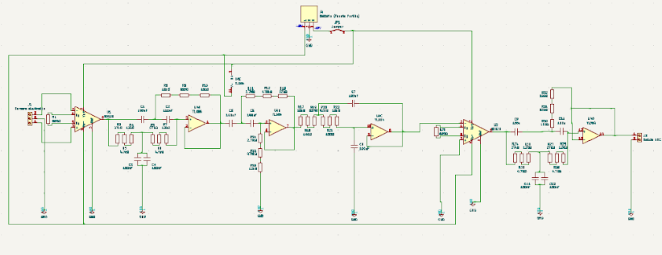
\includegraphics[width=1\linewidth]{Imagenes/Filtros/filtroseeg.png}
    \caption{Esquemático de los filtros del EEG}
\end{figure}

\subsubsection{Esquemático del sistema de control}
\begin{figure}[H]
    \centering
    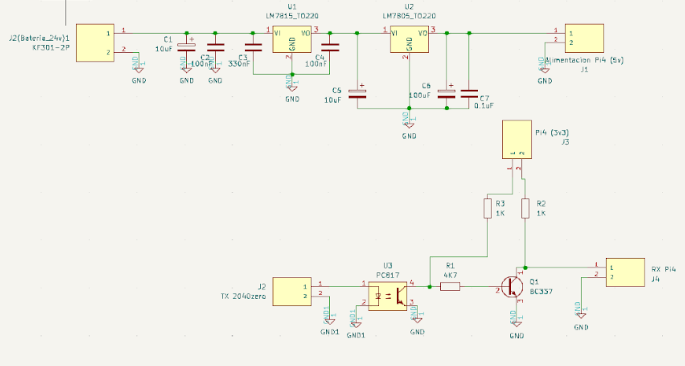
\includegraphics[width=1\linewidth]{Imagenes/SistemaControl/sistemadecontrol.png}
    \caption{Esquemáticos del sistema de control}
\end{figure}

\subsubsection{Esquemático del sistema Offset}
\begin{figure}[H]
    \centering
    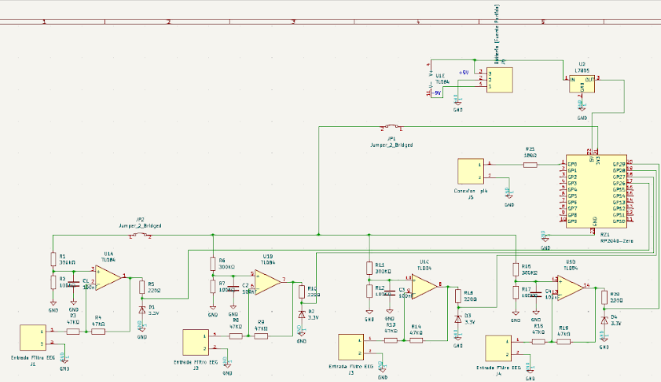
\includegraphics[width=1\linewidth]{Imagenes/SistemaOffset/sistemaoffset.png}
    \caption{Esquemático del sistema de Offset}
\end{figure}

\subsubsection{Esquemáticos de los Puentes H}
\begin{figure}[H]
    \centering
     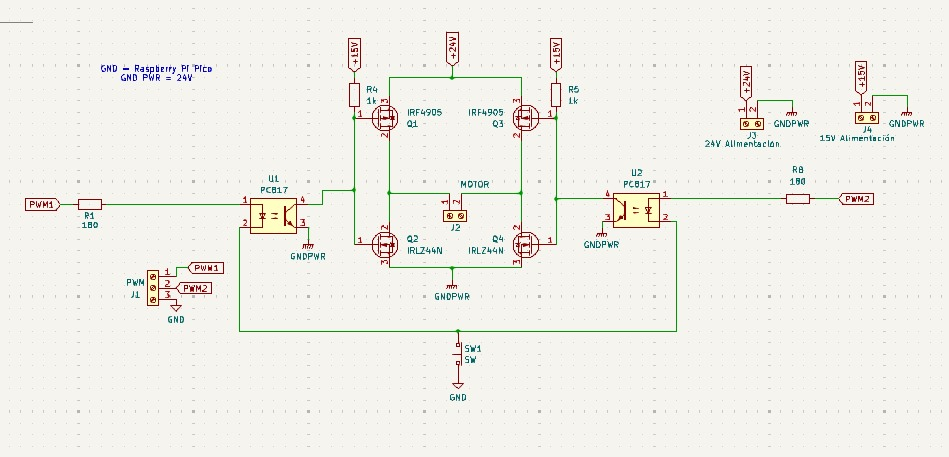
\includegraphics[width=1\textwidth]{Imagenes/PuenteH/WhatsApp Image 2024-08-28 at 9.05.56 AM.jpeg}
    \caption{Puente H (Un Motor)}
\end{figure}

\subsubsection{Esquemático del sistema de emergencia}
\begin{figure}[H]
    \centering
    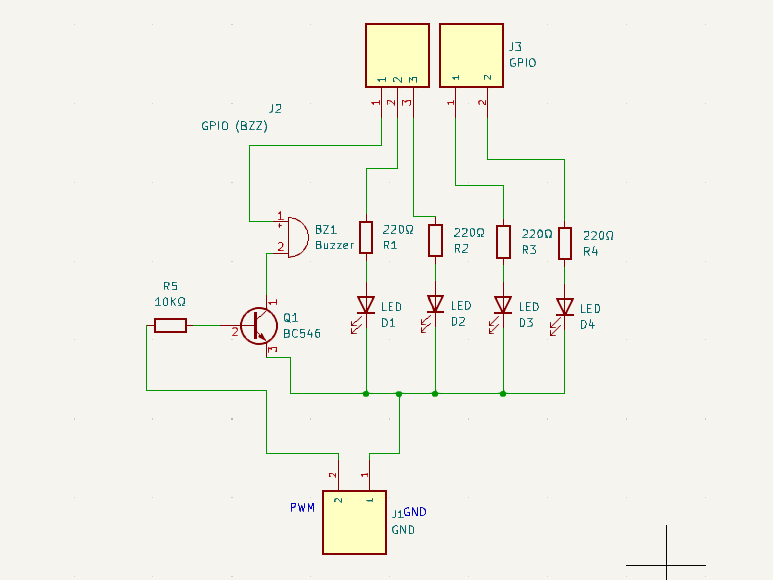
\includegraphics[width=1\textwidth]{Imagenes/SistemaEmergencia/sistemergencia.png}
    \caption{Esquemático del sistema de emegencia}


    \begin{subfigure}[t]{0.5\textwidth}
        \centering
        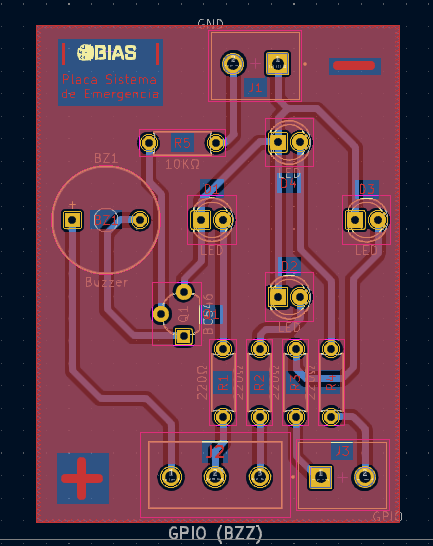
\includegraphics[width=0.5\textwidth]{Imagenes/SistemaEmergencia/sistemergenciapcb.png}
        \caption{PCB Del sistema de emergencia}
    \end{subfigure}%
    ~ 
    \begin{subfigure}[t]{0.5\textwidth}
        \centering
        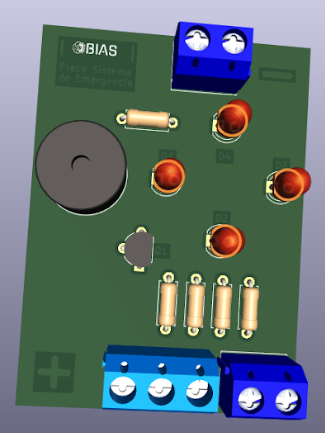
\includegraphics[width=0.5\textwidth]{Imagenes/SistemaEmergencia/sistemergencia3d.png}
        \caption{Modelo 3D Del sistema de emergencia}
    \end{subfigure}

\end{figure}


\newpage

\section{Agradecimientos}
Queremos expresar nuestro más profundo agradecimiento a los profesores que nos han brindado su invaluable apoyo en la realización de este proyecto:

\begin{itemize}

    \item Fabrizio Carlassara: Su asistencia fue crucial en la programación de la mayor parte del proyecto, así como en la creación de circuitos y esquemáticos, la búsqueda de materiales y el desarrollo de los filtros necesarios.


    \item Sergio Medina: Nos brindó su experiencia en la presentación y comercialización del proyecto, además de colaborar en la programación, la búsqueda de materiales y la planificación de los puentes H.


    \item Carlos Bianco: Su apoyo fue esencial en las pruebas y acondicionamiento de los motores, proporcionándonos herramientas y baterías para dichas pruebas, además de colaborar en la búsqueda de materiales.


    \item Daniel Espósito: Nos proporcionó motores y materiales, además de enseñarnos a construir los puentes H para los motores y nos ayudó a solucionar problemas con las pistas de los circuitos para las altas corrientes.

    \item Federico Solomiewicz: Colaboró principalmente en el desarrollo de los filtros, proporcionándonos herramientas para el proyecto y estando siempre disponible para resolver cualquier duda que surgiera.


    \item Juan Carlos Ruiz: Su colaboración fue esencial en las pruebas de los motores para la silla de ruedas, además de ayudarnos principalmente en la creación de los puentes H para los motores y sus circuitos impresos.

\end{itemize}
\end{document}
